 \documentclass{article}
\usepackage[utf8]{inputenc}
\usepackage[a4paper, total={7in, 10in}]{geometry}
\usepackage{braket}
\usepackage{xcolor}
\usepackage{amsmath}
\usepackage{amssymb}
\usepackage{amsfonts}
\usepackage{graphicx}
\usepackage{svg}
\usepackage{float}
\usepackage{tikz}
\usepackage[ruled,vlined]{algorithm2e}
\usepackage{multicol}
\usepackage[backend=biber,style=alphabetic,sorting=ynt]{biblatex}
\usepackage{xcolor}
%\addbibresource{sample.bib} %Import the bibliography file

\newcommand{\commentt}[1]{\textcolor{blue}{ \textbf{[COMMENT]} #1}}
\newcommand{\ctt}[1]{\commentt{#1}}
\newcommand{\prb}[1]{ \mathbf{Pr} \left[ {#1} \right]}
\newcommand{\onotation}[1]{\(\mathcal{O} \left( {#1}  \right) \)}
\newcommand{\ona}[1]{\onotation{#1}}
\newcommand{\PSI}{{\ket{\psi}}}
\newcommand{\LESn}{\ket{\psi_n}}
\newcommand{\LESa}{\ket{\phi_n}}
\newcommand{\LESs}{\frac{1}{\sqrt{n}}\sum_{i}{\ket{\left(0^{i}10^{n-i}\right)^{n}}}}
\newcommand{\Hn}{\mathcal{H}_{n}}
\newcommand{\Ep}{\frac{1}{\sqrt{2^n}}\sum^{2^n}_{x}{ \ket{xx}}}
\newcommand{\HON}{\ket{\psi_{\text{honest}}}}
\newcommand{\Lemma}{\paragraph{Lemma.}}


\setlength{\columnsep}{0.6cm}

\newcommand{\Gz}{ G_{z}^{\delta} } 

\begin{document}

\title{Quantum LTC With Positive Rate}
\author{David Ponarovsky}
\maketitle
\begin{multicols*}{2}
\newcommand{ \Hw }{ \delta\Delta -\Delta^{\frac{1}{2}-\varepsilon}/\delta  }
	\newcommand{ \Nw }{ \Delta^{\frac{3}{2}-\varepsilon}} 
	  \newcommand{ \Gu } { \Gamma^{\cup} }
	  \newcommand{ \Guq } { \Gamma^{\cup, \square} }

    	\newcommand{ \Gsa } {\Gamma_{\square_{1}} }
	\newcommand{ \Gsb } {\Gamma_{\square_{2}} }
        \newcommand{ \Aa } { C_{A_{1}}}  
	\newcommand{ \Ab } { C_{A_{2}}}
	\newcommand{ \Ac } { C_{A_{3}}}
	\newcommand{ \Aab } { \Aa \otimes \Ab } 
	\newcommand{ \Aac } { \Aa \otimes \Ac }
	\newcommand{ \Aabc } { \Aa \otimes \Ab \otimes \Ac }
	\newcommand{ \Aabp } { \Aa^{\perp} \otimes \Ab^{\perp} } 
	\newcommand{ \Aacp } { \Aa^{\perp} \otimes \Ac^{\perp} }
	\newcommand{ \Aabcp } { \Aa^{\perp} \otimes \Ab^{\perp} \otimes \Ac^{\perp} }
	\newcommand{ \Aabpp } { \left( \Aabp \right)^\perp } 
	\newcommand{ \Aacpp } { \left( \Aacp \right)^\perp }
	\newcommand{ \Aabcpp } { \left( \Aabcp \right)^\perp }
	\newcommand{ \YY } {  y_{1}y_{2}^{\top} }
	\newcommand{ \ZZ } {  z_{1}z_{2}^{\top} } 
	\newcommand{ \TT } { \tilde{\tau} } 


  \paragraph{preamble.} preamble.  
  \begin{figure}[H]
            %\label{fig:square}
            \begin{center}
            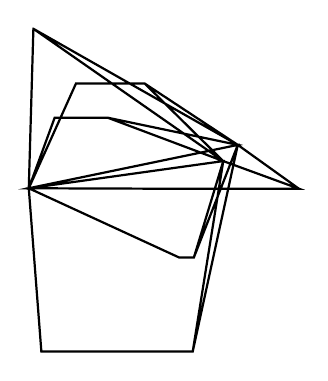
\begin{tikzpicture}
            \draw[thick](0,0)(0,0)  -- (0.3287254933014001, 0.8963121210113115) -- (1.0011951708884037, 0.8963121210113115) -- (2.654391893082545,0.5506424753070788) -- (0,0) -- (0,0)  -- (1.7012736508793056, -0.005753818279713441) -- (3.4306647432585717, -0.005753818279713441) -- (2.654391893082545,0.5506424753070788) -- (0,0) -- 
(0,0)  -- (0.3287254933014001, 0.8963121210113115) -- (1.0011951708884037, 0.8963121210113115) -- (2.654391893082545,0.5506424753070788) -- (0,0) -- (0,0)  -- (0.15966250021255557, -2.0722316584356726) -- (2.082360291368117, -2.0722316584356726) -- (2.654391893082545,0.5506424753070788) -- (0,0) -- 
(0,0)  -- (0.3287254933014001, 0.8963121210113115) -- (1.0011951708884037, 0.8963121210113115) -- (2.654391893082545,0.5506424753070788) -- (0,0) -- (0,0)  -- (1.9104565613922833, -0.879867673900728) -- (2.0964855464386103, -0.879867673900728) -- (2.654391893082545,0.5506424753070788) -- (0,0) -- 
(0,0)  -- (0.0585501944473934, 2.0253698321034452) -- (0.05857810455221624, 2.0253698321034452) -- (2.654391893082545,0.5506424753070788) -- (0,0) -- (0,0)  -- (1.7012736508793056, -0.005753818279713441) -- (3.4306647432585717, -0.005753818279713441) -- (2.654391893082545,0.5506424753070788) -- (0,0) -- 
(0,0)  -- (0.0585501944473934, 2.0253698321034452) -- (0.05857810455221624, 2.0253698321034452) -- (2.654391893082545,0.5506424753070788) -- (0,0) -- (0,0)  -- (0.15966250021255557, -2.0722316584356726) -- (2.082360291368117, -2.0722316584356726) -- (2.654391893082545,0.5506424753070788) -- (0,0) -- 
(0,0)  -- (0.0585501944473934, 2.0253698321034452) -- (0.05857810455221624, 2.0253698321034452) -- (2.654391893082545,0.5506424753070788) -- (0,0) -- (0,0)  -- (1.9104565613922833, -0.879867673900728) -- (2.0964855464386103, -0.879867673900728) -- (2.654391893082545,0.5506424753070788) -- (0,0) -- 
(0,0)  -- (0.599003773610338, 1.3298467713205588) -- (1.472441557291233, 1.3298467713205588) -- (2.654391893082545,0.5506424753070788) -- (0,0) -- (0,0)  -- (1.7012736508793056, -0.005753818279713441) -- (3.4306647432585717, -0.005753818279713441) -- (2.654391893082545,0.5506424753070788) -- (0,0) -- 
(0,0)  -- (0.599003773610338, 1.3298467713205588) -- (1.472441557291233, 1.3298467713205588) -- (2.654391893082545,0.5506424753070788) -- (0,0) -- (0,0)  -- (0.15966250021255557, -2.0722316584356726) -- (2.082360291368117, -2.0722316584356726) -- (2.654391893082545,0.5506424753070788) -- (0,0) -- 
(0,0)  -- (0.599003773610338, 1.3298467713205588) -- (1.472441557291233, 1.3298467713205588) -- (2.654391893082545,0.5506424753070788) -- (0,0) -- (0,0)  -- (1.9104565613922833, -0.879867673900728) -- (2.0964855464386103, -0.879867673900728) -- (2.654391893082545,0.5506424753070788) -- (0,0) -- 
(0,0)  -- (0.3287254933014001, 0.8963121210113115) -- (1.0011951708884037, 0.8963121210113115) -- (2.4699289553294816,0.3450266814858388) -- (0,0) -- (0,0)  -- (1.7012736508793056, -0.005753818279713441) -- (3.4306647432585717, -0.005753818279713441) -- (2.4699289553294816,0.3450266814858388) -- (0,0) -- 
(0,0)  -- (0.3287254933014001, 0.8963121210113115) -- (1.0011951708884037, 0.8963121210113115) -- (2.4699289553294816,0.3450266814858388) -- (0,0) -- (0,0)  -- (0.15966250021255557, -2.0722316584356726) -- (2.082360291368117, -2.0722316584356726) -- (2.4699289553294816,0.3450266814858388) -- (0,0) -- 
(0,0)  -- (0.3287254933014001, 0.8963121210113115) -- (1.0011951708884037, 0.8963121210113115) -- (2.4699289553294816,0.3450266814858388) -- (0,0) -- (0,0)  -- (1.9104565613922833, -0.879867673900728) -- (2.0964855464386103, -0.879867673900728) -- (2.4699289553294816,0.3450266814858388) -- (0,0) -- 
(0,0)  -- (0.0585501944473934, 2.0253698321034452) -- (0.05857810455221624, 2.0253698321034452) -- (2.4699289553294816,0.3450266814858388) -- (0,0) -- (0,0)  -- (1.7012736508793056, -0.005753818279713441) -- (3.4306647432585717, -0.005753818279713441) -- (2.4699289553294816,0.3450266814858388) -- (0,0) -- 
(0,0)  -- (0.0585501944473934, 2.0253698321034452) -- (0.05857810455221624, 2.0253698321034452) -- (2.4699289553294816,0.3450266814858388) -- (0,0) -- (0,0)  -- (0.15966250021255557, -2.0722316584356726) -- (2.082360291368117, -2.0722316584356726) -- (2.4699289553294816,0.3450266814858388) -- (0,0) -- 
(0,0)  -- (0.0585501944473934, 2.0253698321034452) -- (0.05857810455221624, 2.0253698321034452) -- (2.4699289553294816,0.3450266814858388) -- (0,0) -- (0,0)  -- (1.9104565613922833, -0.879867673900728) -- (2.0964855464386103, -0.879867673900728) -- (2.4699289553294816,0.3450266814858388) -- (0,0) -- 
(0,0)  -- (0.599003773610338, 1.3298467713205588) -- (1.472441557291233, 1.3298467713205588) -- (2.4699289553294816,0.3450266814858388) -- (0,0) -- (0,0)  -- (1.7012736508793056, -0.005753818279713441) -- (3.4306647432585717, -0.005753818279713441) -- (2.4699289553294816,0.3450266814858388) -- (0,0) -- 
(0,0)  -- (0.599003773610338, 1.3298467713205588) -- (1.472441557291233, 1.3298467713205588) -- (2.4699289553294816,0.3450266814858388) -- (0,0) -- (0,0)  -- (0.15966250021255557, -2.0722316584356726) -- (2.082360291368117, -2.0722316584356726) -- (2.4699289553294816,0.3450266814858388) -- (0,0) -- 
(0,0)  -- (0.599003773610338, 1.3298467713205588) -- (1.472441557291233, 1.3298467713205588) -- (2.4699289553294816,0.3450266814858388) -- (0,0) -- (0,0)  -- (1.9104565613922833, -0.879867673900728) -- (2.0964855464386103, -0.879867673900728) -- (2.4699289553294816,0.3450266814858388) -- (0,0) -- 
(0,0);
            \end{tikzpicture}
            \end{center}
            \caption{Square of the complex, with edges $(g,ag), (agb, gb) \in E_A,
            (g,gb), (agb, ag) \in E_B.$ \label{fig:square}
            }
            \end{figure}
 \begin{figure}[H]
            %\label{fig:square}
            \begin{center}
            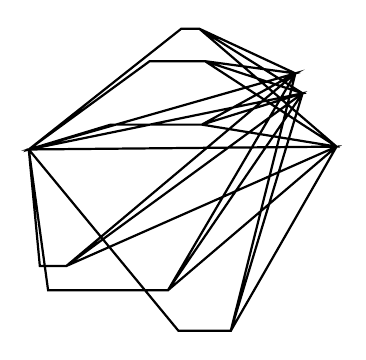
\begin{tikzpicture}
            \draw[thick](0,0)(0,0)  -- (1.535372347311892, 1.1213298021631504) -- (2.2379794851961012, 1.1213298021631504) -- (3.476997659509289,0.7135038838308749) -- (0,0) -- (0,0)  -- (0.1404230138849485, -1.480057005293598) -- (0.4762988367361829, -1.480057005293598) -- (3.476997659509289,0.7135038838308749) -- (0,0) -- 
(0,0)  -- (1.535372347311892, 1.1213298021631504) -- (2.2379794851961012, 1.1213298021631504) -- (3.476997659509289,0.7135038838308749) -- (0,0) -- (0,0)  -- (1.901280110802629, -2.3032744599101562) -- (2.56547162986633, -2.3032744599101562) -- (3.476997659509289,0.7135038838308749) -- (0,0) -- 
(0,0)  -- (1.535372347311892, 1.1213298021631504) -- (2.2379794851961012, 1.1213298021631504) -- (3.476997659509289,0.7135038838308749) -- (0,0) -- (0,0)  -- (0.24526389584864194, -1.7875006447013235) -- (1.768260303605214, -1.7875006447013235) -- (3.476997659509289,0.7135038838308749) -- (0,0) -- 
(0,0)  -- (1.9359288263462426, 1.5327874660287055) -- (2.166961628754121, 1.5327874660287055) -- (3.476997659509289,0.7135038838308749) -- (0,0) -- (0,0)  -- (0.1404230138849485, -1.480057005293598) -- (0.4762988367361829, -1.480057005293598) -- (3.476997659509289,0.7135038838308749) -- (0,0) -- 
(0,0)  -- (1.9359288263462426, 1.5327874660287055) -- (2.166961628754121, 1.5327874660287055) -- (3.476997659509289,0.7135038838308749) -- (0,0) -- (0,0)  -- (1.901280110802629, -2.3032744599101562) -- (2.56547162986633, -2.3032744599101562) -- (3.476997659509289,0.7135038838308749) -- (0,0) -- 
(0,0)  -- (1.9359288263462426, 1.5327874660287055) -- (2.166961628754121, 1.5327874660287055) -- (3.476997659509289,0.7135038838308749) -- (0,0) -- (0,0)  -- (0.24526389584864194, -1.7875006447013235) -- (1.768260303605214, -1.7875006447013235) -- (3.476997659509289,0.7135038838308749) -- (0,0) -- 
(0,0)  -- (1.0410241205696322, 0.3157009485436315) -- (2.1977592978559883, 0.3157009485436315) -- (3.476997659509289,0.7135038838308749) -- (0,0) -- (0,0)  -- (0.1404230138849485, -1.480057005293598) -- (0.4762988367361829, -1.480057005293598) -- (3.476997659509289,0.7135038838308749) -- (0,0) -- 
(0,0)  -- (1.0410241205696322, 0.3157009485436315) -- (2.1977592978559883, 0.3157009485436315) -- (3.476997659509289,0.7135038838308749) -- (0,0) -- (0,0)  -- (1.901280110802629, -2.3032744599101562) -- (2.56547162986633, -2.3032744599101562) -- (3.476997659509289,0.7135038838308749) -- (0,0) -- 
(0,0)  -- (1.0410241205696322, 0.3157009485436315) -- (2.1977592978559883, 0.3157009485436315) -- (3.476997659509289,0.7135038838308749) -- (0,0) -- (0,0)  -- (0.24526389584864194, -1.7875006447013235) -- (1.768260303605214, -1.7875006447013235) -- (3.476997659509289,0.7135038838308749) -- (0,0) -- 
(0,0)  -- (1.535372347311892, 1.1213298021631504) -- (2.2379794851961012, 1.1213298021631504) -- (3.9085316658754827,0.03618677560008394) -- (0,0) -- (0,0)  -- (0.1404230138849485, -1.480057005293598) -- (0.4762988367361829, -1.480057005293598) -- (3.9085316658754827,0.03618677560008394) -- (0,0) -- 
(0,0)  -- (1.535372347311892, 1.1213298021631504) -- (2.2379794851961012, 1.1213298021631504) -- (3.9085316658754827,0.03618677560008394) -- (0,0) -- (0,0)  -- (1.901280110802629, -2.3032744599101562) -- (2.56547162986633, -2.3032744599101562) -- (3.9085316658754827,0.03618677560008394) -- (0,0) -- 
(0,0)  -- (1.535372347311892, 1.1213298021631504) -- (2.2379794851961012, 1.1213298021631504) -- (3.9085316658754827,0.03618677560008394) -- (0,0) -- (0,0)  -- (0.24526389584864194, -1.7875006447013235) -- (1.768260303605214, -1.7875006447013235) -- (3.9085316658754827,0.03618677560008394) -- (0,0) -- 
(0,0)  -- (1.9359288263462426, 1.5327874660287055) -- (2.166961628754121, 1.5327874660287055) -- (3.9085316658754827,0.03618677560008394) -- (0,0) -- (0,0)  -- (0.1404230138849485, -1.480057005293598) -- (0.4762988367361829, -1.480057005293598) -- (3.9085316658754827,0.03618677560008394) -- (0,0) -- 
(0,0)  -- (1.9359288263462426, 1.5327874660287055) -- (2.166961628754121, 1.5327874660287055) -- (3.9085316658754827,0.03618677560008394) -- (0,0) -- (0,0)  -- (1.901280110802629, -2.3032744599101562) -- (2.56547162986633, -2.3032744599101562) -- (3.9085316658754827,0.03618677560008394) -- (0,0) -- 
(0,0)  -- (1.9359288263462426, 1.5327874660287055) -- (2.166961628754121, 1.5327874660287055) -- (3.9085316658754827,0.03618677560008394) -- (0,0) -- (0,0)  -- (0.24526389584864194, -1.7875006447013235) -- (1.768260303605214, -1.7875006447013235) -- (3.9085316658754827,0.03618677560008394) -- (0,0) -- 
(0,0)  -- (1.0410241205696322, 0.3157009485436315) -- (2.1977592978559883, 0.3157009485436315) -- (3.9085316658754827,0.03618677560008394) -- (0,0) -- (0,0)  -- (0.1404230138849485, -1.480057005293598) -- (0.4762988367361829, -1.480057005293598) -- (3.9085316658754827,0.03618677560008394) -- (0,0) -- 
(0,0)  -- (1.0410241205696322, 0.3157009485436315) -- (2.1977592978559883, 0.3157009485436315) -- (3.9085316658754827,0.03618677560008394) -- (0,0) -- (0,0)  -- (1.901280110802629, -2.3032744599101562) -- (2.56547162986633, -2.3032744599101562) -- (3.9085316658754827,0.03618677560008394) -- (0,0) -- 
(0,0)  -- (1.0410241205696322, 0.3157009485436315) -- (2.1977592978559883, 0.3157009485436315) -- (3.9085316658754827,0.03618677560008394) -- (0,0) -- (0,0)  -- (0.24526389584864194, -1.7875006447013235) -- (1.768260303605214, -1.7875006447013235) -- (3.9085316658754827,0.03618677560008394) -- (0,0) -- 
(0,0)  -- (1.535372347311892, 1.1213298021631504) -- (2.2379794851961012, 1.1213298021631504) -- (3.385528117814252,0.9663763317526646) -- (0,0) -- (0,0)  -- (0.1404230138849485, -1.480057005293598) -- (0.4762988367361829, -1.480057005293598) -- (3.385528117814252,0.9663763317526646) -- (0,0) -- 
(0,0)  -- (1.535372347311892, 1.1213298021631504) -- (2.2379794851961012, 1.1213298021631504) -- (3.385528117814252,0.9663763317526646) -- (0,0) -- (0,0)  -- (1.901280110802629, -2.3032744599101562) -- (2.56547162986633, -2.3032744599101562) -- (3.385528117814252,0.9663763317526646) -- (0,0) -- 
(0,0)  -- (1.535372347311892, 1.1213298021631504) -- (2.2379794851961012, 1.1213298021631504) -- (3.385528117814252,0.9663763317526646) -- (0,0) -- (0,0)  -- (0.24526389584864194, -1.7875006447013235) -- (1.768260303605214, -1.7875006447013235) -- (3.385528117814252,0.9663763317526646) -- (0,0) -- 
(0,0)  -- (1.9359288263462426, 1.5327874660287055) -- (2.166961628754121, 1.5327874660287055) -- (3.385528117814252,0.9663763317526646) -- (0,0) -- (0,0)  -- (0.1404230138849485, -1.480057005293598) -- (0.4762988367361829, -1.480057005293598) -- (3.385528117814252,0.9663763317526646) -- (0,0) -- 
(0,0)  -- (1.9359288263462426, 1.5327874660287055) -- (2.166961628754121, 1.5327874660287055) -- (3.385528117814252,0.9663763317526646) -- (0,0) -- (0,0)  -- (1.901280110802629, -2.3032744599101562) -- (2.56547162986633, -2.3032744599101562) -- (3.385528117814252,0.9663763317526646) -- (0,0) -- 
(0,0)  -- (1.9359288263462426, 1.5327874660287055) -- (2.166961628754121, 1.5327874660287055) -- (3.385528117814252,0.9663763317526646) -- (0,0) -- (0,0)  -- (0.24526389584864194, -1.7875006447013235) -- (1.768260303605214, -1.7875006447013235) -- (3.385528117814252,0.9663763317526646) -- (0,0) -- 
(0,0)  -- (1.0410241205696322, 0.3157009485436315) -- (2.1977592978559883, 0.3157009485436315) -- (3.385528117814252,0.9663763317526646) -- (0,0) -- (0,0)  -- (0.1404230138849485, -1.480057005293598) -- (0.4762988367361829, -1.480057005293598) -- (3.385528117814252,0.9663763317526646) -- (0,0) -- 
(0,0)  -- (1.0410241205696322, 0.3157009485436315) -- (2.1977592978559883, 0.3157009485436315) -- (3.385528117814252,0.9663763317526646) -- (0,0) -- (0,0)  -- (1.901280110802629, -2.3032744599101562) -- (2.56547162986633, -2.3032744599101562) -- (3.385528117814252,0.9663763317526646) -- (0,0) -- 
(0,0)  -- (1.0410241205696322, 0.3157009485436315) -- (2.1977592978559883, 0.3157009485436315) -- (3.385528117814252,0.9663763317526646) -- (0,0) -- (0,0)  -- (0.24526389584864194, -1.7875006447013235) -- (1.768260303605214, -1.7875006447013235) -- (3.385528117814252,0.9663763317526646) -- (0,0) -- 
(0,0);
            \end{tikzpicture}
            \end{center}
            \caption{Square of the complex, with edges $(g,ag), (agb, gb) \in E_A,
            (g,gb), (agb, ag) \in E_B.$ \label{fig:square}
            }
            \end{figure}
 \begin{figure}[H]
            %\label{fig:square}
            \begin{center}
            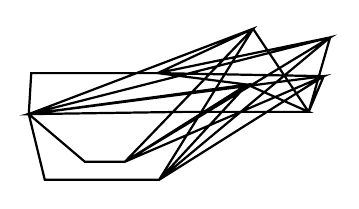
\begin{tikzpicture}
            \draw[thick](0,0)(0,0)  -- (1.9621478034272664, 0.02857998345414836) -- (3.554502393404834, 0.02857998345414836) -- (3.7454939875680617,0.48207337570869907) -- (0,0) -- (0,0)  -- (0.7109200774465665, -0.6037579970947805) -- (1.2219313304070683, -0.6037579970947805) -- (3.7454939875680617,0.48207337570869907) -- (0,0) -- 
(0,0)  -- (1.9621478034272664, 0.02857998345414836) -- (3.554502393404834, 0.02857998345414836) -- (3.7454939875680617,0.48207337570869907) -- (0,0) -- (0,0)  -- (0.20325044682159876, -0.8338083467723957) -- (1.6554396936200904, -0.8338083467723957) -- (3.7454939875680617,0.48207337570869907) -- (0,0) -- 
(0,0)  -- (0.03127912633431462, 0.520882915567774) -- (1.6367893242381326, 0.520882915567774) -- (3.7454939875680617,0.48207337570869907) -- (0,0) -- (0,0)  -- (0.7109200774465665, -0.6037579970947805) -- (1.2219313304070683, -0.6037579970947805) -- (3.7454939875680617,0.48207337570869907) -- (0,0) -- 
(0,0)  -- (0.03127912633431462, 0.520882915567774) -- (1.6367893242381326, 0.520882915567774) -- (3.7454939875680617,0.48207337570869907) -- (0,0) -- (0,0)  -- (0.20325044682159876, -0.8338083467723957) -- (1.6554396936200904, -0.8338083467723957) -- (3.7454939875680617,0.48207337570869907) -- (0,0) -- 
(0,0)  -- (1.9621478034272664, 0.02857998345414836) -- (3.554502393404834, 0.02857998345414836) -- (2.8478676854034033,1.0839157470227356) -- (0,0) -- (0,0)  -- (0.7109200774465665, -0.6037579970947805) -- (1.2219313304070683, -0.6037579970947805) -- (2.8478676854034033,1.0839157470227356) -- (0,0) -- 
(0,0)  -- (1.9621478034272664, 0.02857998345414836) -- (3.554502393404834, 0.02857998345414836) -- (2.8478676854034033,1.0839157470227356) -- (0,0) -- (0,0)  -- (0.20325044682159876, -0.8338083467723957) -- (1.6554396936200904, -0.8338083467723957) -- (2.8478676854034033,1.0839157470227356) -- (0,0) -- 
(0,0)  -- (0.03127912633431462, 0.520882915567774) -- (1.6367893242381326, 0.520882915567774) -- (2.8478676854034033,1.0839157470227356) -- (0,0) -- (0,0)  -- (0.7109200774465665, -0.6037579970947805) -- (1.2219313304070683, -0.6037579970947805) -- (2.8478676854034033,1.0839157470227356) -- (0,0) -- 
(0,0)  -- (0.03127912633431462, 0.520882915567774) -- (1.6367893242381326, 0.520882915567774) -- (2.8478676854034033,1.0839157470227356) -- (0,0) -- (0,0)  -- (0.20325044682159876, -0.8338083467723957) -- (1.6554396936200904, -0.8338083467723957) -- (2.8478676854034033,1.0839157470227356) -- (0,0) -- 
(0,0)  -- (1.9621478034272664, 0.02857998345414836) -- (3.554502393404834, 0.02857998345414836) -- (2.772783795505795,0.3751589227254338) -- (0,0) -- (0,0)  -- (0.7109200774465665, -0.6037579970947805) -- (1.2219313304070683, -0.6037579970947805) -- (2.772783795505795,0.3751589227254338) -- (0,0) -- 
(0,0)  -- (1.9621478034272664, 0.02857998345414836) -- (3.554502393404834, 0.02857998345414836) -- (2.772783795505795,0.3751589227254338) -- (0,0) -- (0,0)  -- (0.20325044682159876, -0.8338083467723957) -- (1.6554396936200904, -0.8338083467723957) -- (2.772783795505795,0.3751589227254338) -- (0,0) -- 
(0,0)  -- (0.03127912633431462, 0.520882915567774) -- (1.6367893242381326, 0.520882915567774) -- (2.772783795505795,0.3751589227254338) -- (0,0) -- (0,0)  -- (0.7109200774465665, -0.6037579970947805) -- (1.2219313304070683, -0.6037579970947805) -- (2.772783795505795,0.3751589227254338) -- (0,0) -- 
(0,0)  -- (0.03127912633431462, 0.520882915567774) -- (1.6367893242381326, 0.520882915567774) -- (2.772783795505795,0.3751589227254338) -- (0,0) -- (0,0)  -- (0.20325044682159876, -0.8338083467723957) -- (1.6554396936200904, -0.8338083467723957) -- (2.772783795505795,0.3751589227254338) -- (0,0) -- 
(0,0)  -- (1.9621478034272664, 0.02857998345414836) -- (3.554502393404834, 0.02857998345414836) -- (3.826702545809641,0.974103404069246) -- (0,0) -- (0,0)  -- (0.7109200774465665, -0.6037579970947805) -- (1.2219313304070683, -0.6037579970947805) -- (3.826702545809641,0.974103404069246) -- (0,0) -- 
(0,0)  -- (1.9621478034272664, 0.02857998345414836) -- (3.554502393404834, 0.02857998345414836) -- (3.826702545809641,0.974103404069246) -- (0,0) -- (0,0)  -- (0.20325044682159876, -0.8338083467723957) -- (1.6554396936200904, -0.8338083467723957) -- (3.826702545809641,0.974103404069246) -- (0,0) -- 
(0,0)  -- (0.03127912633431462, 0.520882915567774) -- (1.6367893242381326, 0.520882915567774) -- (3.826702545809641,0.974103404069246) -- (0,0) -- (0,0)  -- (0.7109200774465665, -0.6037579970947805) -- (1.2219313304070683, -0.6037579970947805) -- (3.826702545809641,0.974103404069246) -- (0,0) -- 
(0,0)  -- (0.03127912633431462, 0.520882915567774) -- (1.6367893242381326, 0.520882915567774) -- (3.826702545809641,0.974103404069246) -- (0,0) -- (0,0)  -- (0.20325044682159876, -0.8338083467723957) -- (1.6554396936200904, -0.8338083467723957) -- (3.826702545809641,0.974103404069246) -- (0,0) -- 
(0,0);
            \end{tikzpicture}
            \end{center}
            \caption{Square of the complex, with edges $(g,ag), (agb, gb) \in E_A,
            (g,gb), (agb, ag) \in E_B.$ \label{fig:square}
            }
            \end{figure}
 
\end{multicols*}
  % \printbibliography 
\end{document}

 